\documentclass[11pt,a4paper]{article}

\usepackage[applemac]{inputenc}
\usepackage{latexsym}
\usepackage{graphicx}
\usepackage[english]{babel}
\usepackage{amsmath,amssymb}
\usepackage{calc}
\usepackage{multicol}
\usepackage{fancyhdr}
\usepackage{lastpage}
\usepackage[T1]{fontenc}
\usepackage{stmaryrd}
\usepackage[]{algorithm2e}
\usepackage{float}


\begin{document}

\begin{titlepage}
	\title{Optimistic approaches in Contextual Linear Bandit models}
	\author{Mathurin \textsc{Massias} \and Cl�ment \textsc{Nicolle}}
	\date{\today} 
	\maketitle
	\thispagestyle{empty}
	\tableofcontents
\hspace{-6mm}
\end{titlepage}
\newpage
\pagestyle{plain}

\section*{Introduction}

The $K$ multi-armed bandit with partial observation setting is well-studied: at each time $t$, an agent is presented with a fixed set of $K$ arms, from which he chooses one to draw, get a reward $r_t$ (without knowing the rewards he would have obtained pulling another arm), and moves on to $t+1$. The goal of the agent is to maximize its cumulated reward, or to minimize the difference with the cumulated reward he would have had if he had always pulled the best arm.
%
\\[5mm]Here we study a contextual bandit problem, meaning that the set of arms the agent can pull might change over time. For example, we may consider the case of a newspaper website which recommends articles to a user. The arm which is pulled corresponds to the article which is suggested in first position, and the reward depends on if the user clicks on this suggestion. This problem is contextual because over time, the set of available articles can change, and the popularity of an article is likely to decrease as time goes by.
%
\\[5mm]In our problem, we consider that each arm can be described by a vector of $d \in \mathbb{N}^*$ features, which is fixed. In the previous newspaper website example, these features could be the frequencies of some words.
%
\\[3mm]What's more, we study a linear bandit problem: we assume that there exists $\theta \in R^d$ (the same for all arms) such that the reward for pulling arm $i$ at time $t$ is $\theta^{\top} x_i + \epsilon_{t}$, where $\epsilon$ is a centered Gaussian noise. Since the noise is uncontrollable, the algorithms focus on estimating $\theta$, to choose the arm with maximal expected reward $\theta^{\top}x_i$.
\\We consider that $\theta$ is normalized, to simplify the computation of the upper confidence bound. $x_a$s are also normalized, so that adding noise has the same effect on all of them.
%
\\[3mm]To model the change in the set of arms over time, we consider that at each iteration the agent cannot choose amongst all the arms, but only from a fraction of them (denoted $\mathcal{A}_t$, which changes at each iteration, whose cardinal $K$ is a fixed parameter). 
%
\\[5mm]For all our implementations, unless otherwise specified, we have chosen the following parameters :
\\- horizon: $T =10,000$ draws
\\- dimension of the feature space: $d = 100$
\\- total number of arms: $N = 1,000$
\\- number of arms the agent can pull from at each time $t$: $K = 100$
\\- probability that the considered concentration inequality holds: $\delta = 0.05$
\\- seed for all our generators, so the results are reproducible and algorithms can be compared: $s = 1$
%
\\[5mm]The best arm is number 912, giving $0.98$ on average. The repartition of the $N$ mean rewards is as follow:
\begin{figure}[H]
\centering
\noindent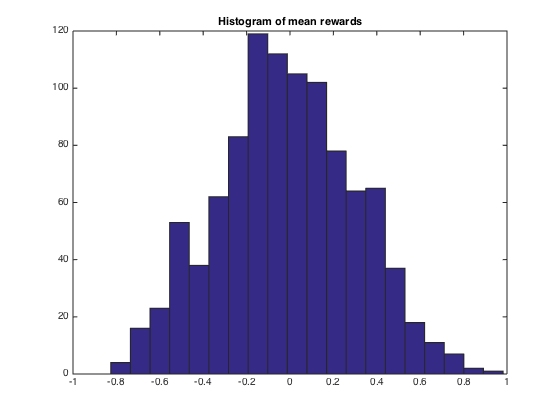
\includegraphics[scale=0.4]{hist_mean_rewards.png}
\caption{Histogram of mean rewards for our 1,000 arms}
\end{figure}
%
\vspace{5mm}What we call regret at iteration $t$ is sometimes called \emph{pseudo-regret} : ${\theta^{\top}(x_{a_t^*} - x_{a_t})}$ where $a_t$ was the arm pulled and $a_t^*$ was the arm maximizing the expected reward (${a_t^* = \mathrm{argmax}_{a \in \mathcal{A}_t} (\theta^{\top} x_a)}$).
\\Since the noise is centered, our regret is just the expectation of the difference between the maximum reward and the reward received. Considering this \emph{pseudo-regret} makes sense: if the noise is independent of the arm selected ($\epsilon_{a,t} = \epsilon_a$), then the noise term cancels out in this difference.
\section{Presentation of LinUCB}

\subsection{Principle}

In all bandit problems, there is a trade-off between exploitation and exploration: to minimize his cumulative regret, the agent must pull the best arm (exploitation), but to do so he must know the best arm (exploration). Pulling all arms uniformly results in a very good knowledge of their distributions, but in poor exploitation, while always pulling the arm which appears best so far ('naive' algorithm) performs badly too, because the best arm can give a poor reward the first time, and never be pulled again.
%
\\[5mm]LinUCB (Linear Upper Confidence Bound) algorithm is derived from the non-contextual algorithm UCB. It is an optimistic algorithm, because it chooses the arms which has the highest upper confidence bound for its mean reward, $\theta^{\top}x_a$.
%
\\The principle of this algorithm is, at each iteration, to compute an estimate for $\theta$ and an upper confidence bound for each of the available arms (both based on previous observations), then to pull the arm which has the highest UCB, update the observations made so far, and move to next iteration, where a new estimate of $\theta$ is computed, etc.
%
\\At each iteration $t$, the estimate of $\theta$, $\hat{\theta}_t$, is computed using a linear regression: since for all $s$ in $\llbracket 1, t \rrbracket$, we have $x_s^{\top} \theta = r_s$, left-multiplying each side by $x_s$ and summing for all indices from $1$ to $t$, we have 
%
$$(\sum\limits_{1}^{t}  x_s x_s^{\top} ) \theta =   \sum\limits_{1}^{t} r_s x_s$$
which can be written in matricial form $A_t \theta = b_t$.
\\Using this formula, even if the number of iterations grows, $A_t$ and $b_t$ remain of fixed size. At each iteration we update $A_t$, $b_t$ and the estimate $\hat{\theta}_t = A_t^{-1}b_t$. Since inversing $A_t$ in computationally costly, we might update it every $k$ iterations only, and thus use the same $\hat{\theta}_t$ for $k$ consecutive iterations.
%
\\[3mm]Initializing $A$ to $I_d$ corresponds to a ridge regression : indeed, if we denote $D_t$ the $t \times d$ design matrix at iteration $t$ : $D_t = \begin{pmatrix} x_1^{\top} \\ ... \\x_t^{\top} \end{pmatrix}$ and $r_t$ the rewards vector $\begin{pmatrix} r_1 \\ ... \\r_t \end{pmatrix}$ , we have: 
%
$$\hat{\theta}_t= (D_t^{\top} D_t + I_d)^{-1} D_t^{\top} r_t$$
which is the formula for a least square ridge regression with regularization parameter equal to 1.
%TODO influence of this parameter ?
%
\\[5mm]The pseudo-code for LinUCB is the following:
\\[3mm]\begin{algorithm}[H]
 \KwData{bandit $\mathcal{A}$, exploration parameter $\alpha$, $K$, horizon $T$}
 $A_1 = I_d$ \;
 $b_1 = 0$ \;
 \For{$t = 1, 2, \ldots, T$}{
  $\hat{\theta}_t = A_t^{-1} b_t$ \;
  Observe $K$ feature vectors: $(x_a)_{a \in \mathcal{A}_t}$ with $\mathcal{A}_t \subset \mathcal{A}$\;
  \For{$a \in \mathcal{A}_t$}{
    $p_{t,a} = \hat{\theta}_t^{\top} x_a + \alpha \sqrt{x_a^{\top}A_t^{-1} x_a}$
   }
   
   Choose arm with higher UCB: $a^*_t = \mathrm{argmax}_{a \in \mathcal{A}_t} p_{t,a} $ \;
   Observe reward $r_t$ \;
   $A_{t+1} = A_t + x_{a^*_t} x_{a^*_t}^{\top}$ \;
   $b_{t+1} = b_t + r_t x_{a^*_t}$ \;
   }
 
  \KwResult{sequences of actions $(a^*_t)$ and payoffs $(r_t)$, $\hat{\theta}_T$}
 \vspace{5mm}
 \caption{LinUCB algorithm}
\end{algorithm}
%
\vspace{5mm}The code can be found in \texttt{linUCB.m}.
%
\subsection{Computation of the UCB}
Since noise is unpredictable, the algorithm only focuses on the expected reward for an arm, $\theta^{\top} x_a$, or equivalently $x_a^{\top} \theta$.
\\Using the previous notations $D_t$ and $R_t$, the difference between the real and estimated rewards at time $t$ for arm $a \in \mathcal{A}_t$ is:
$$\begin{aligned} x_a^{\top} \hat{\theta}_t - x_a^{\top} \theta &= x_a^{\top} A^{-1}_tb_t - x_a^{\top}A_t^{-1} A_t \theta
\\& = x_a^{\top} A^{-1}_t b_t - x_a^{\top}A_t^{-1} (I_d + D^{\top}_tD_t) \theta
\\& = x_a^{\top} A^{-1}_t b_t - x_a^{\top}A_t^{-1} (I_d + D^{\top}_tD_t) \theta
\\& = x_a^{\top} A^{-1}_t D^{\top}_t R_t- x_a^{\top}A_t^{-1} (\theta + D^{\top}_tD_t \theta)
\\& = x_a^{\top} A^{-1}_t D^{\top}_t (R_t - D_t \theta)- x_a^{\top}A_t^{-1} \theta 
\end{aligned}$$
%
Using triangular inequality, Cauchy-Schwartz inequality, $A_t^{\top} = A_t$ and ${\Vert \theta \Vert = 1}$, we get:
$$ \vert x_a^{\top} \hat{\theta}_t - x_a^{\top} \theta \vert \leq \vert x_a^{\top} A^{-1}_t D^{\top}_t (R_t - D_t \theta) \vert + \Vert A^{-1}_t x_a \Vert $$
%
%TODO one is a variance term, other is bias
%
For the second term, we have 
$$\begin{aligned} 
\Vert A^{-1}_t x_a \Vert^2  &= x^{\top}_a A_t^{-1} I_d A_t^{-1} x_a
\\& \leq x^{\top}_a A_t^{-1} (I_d + D_t^{\top}D_t)A_t^{-1} x_a
\\& \leq x^{\top}_a A_t^{-1} x_a
\end{aligned}$$
%
And for the first one, using $\mathbb{E}[R_t - D_t \theta] = 0$ and Azuma's inequality :
$$\begin{aligned} \mathbb{P}( \vert x_a^{\top} A^{-1}_t D^{\top}_t (R_t - D_t \theta) \vert \geq \alpha \sqrt{x^{\top}_a A_t^{-1} x_a})
& \leq 2 \, \mathrm{exp} (- \frac{2 \alpha^2 x^{\top}_a A_t^{-1} x_a}{\Vert D_tA^{-1}_t x_a \Vert ^2})
\\ &\leq 2 e^{-2 \alpha^2}
\\ &= \delta  % T \,
\end{aligned}$$
Using a union bound for the K possible arms in $\mathcal{A}_t$, we get a uniform bound with probability $1 - \delta$.
\\Combining the bound on the first term and second term, with probability $1 - \delta$, 
$$\vert x_a^{\top} \hat{\theta}_t - x_a^{\top} \theta \vert \leq (1 + \alpha) \sqrt{x^{\top}_a A_t^{-1} x_a}$$
where $\alpha = \sqrt{\frac{\mathrm{log} (2/\delta)}{2}}$.

%
\subsection{Impact of exploration parameter}
The exploration parameter $\alpha$ is related to $\delta$ by $\alpha = 1 + \sqrt{\frac{\mathrm{log \,}(2 / \delta)}{2}}$. As the concentration inequality holds with probability $1 - \delta$, if $\delta \to 0$, then ${\alpha \to \infty}$, meaning that if we want a very high probability to find the observed value in a given set, this set must be very large.
%
The higher $\alpha$, the larger the confidence sets: the algorithm is very 'suspicious' about the value $\hat{\theta}_t^{\top}x_i$, and explores more than with a smaller $\alpha$.
\\On the contrary, $\alpha = 0$ %TODO alpha cannot be lesser than 1 with current formula
corresponds to a naive version, where the arm which is pulled is just the one which has the highest mean of rewards observed so far.
\\[5mm]Here are the regrets obtained for LinUCB, with different $\alpha$s (sampled logarithmically from 0 to 1)

\begin{figure}[H]
\centering
\noindent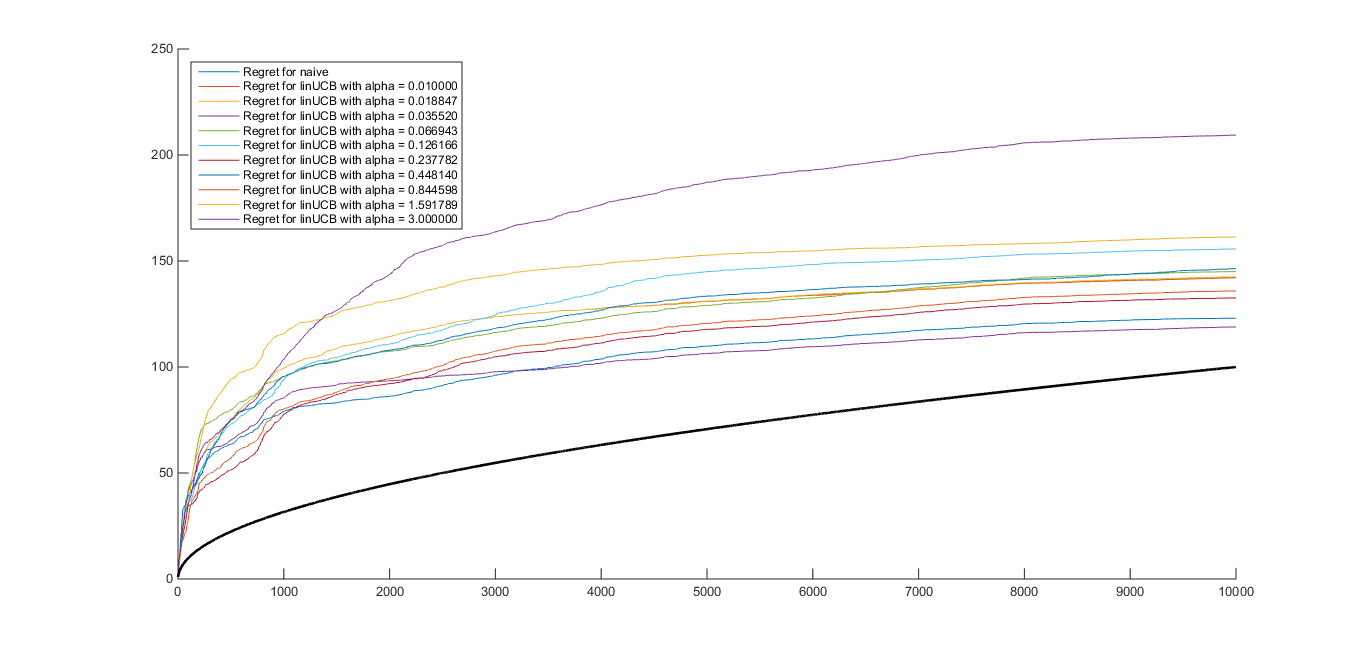
\includegraphics[scale=0.3]{regrets_alphas.png}
\caption{Regret curves for LinUCB with different exploration parameters}
\end{figure}

We figure out one particular trajectory here, but we observe similar results on other draws. We see that the best value for $\alpha$ is $0.036$ here.
%TODO See that low and high alphas perform poorly.
%TODO mention that alpha should change over time.

\subsection{LinUCB for disjoint linear models}	

In the article \textit{A Contextual-Bandit Approach to Personalized News Article Recommendation} $\left[ 1\right]$, the authors consider the case of a disjoint linear model, where we do not have $E[r_{t,a}|x_a] = x_{a}^T \theta^{*}$ anymore, but : $E[r_{t,a}|x_a] = x_{a}^T \theta_a^{*}$, i.e. a different $\theta$ for each possible arm. It is called "disjoint" as we do not have anymore the correlation between the arms.
%
\\Still, we wanted to study the differences with the previous linUCB algorithm. We now simulate a matrix $\theta$, and not a simple value, in which each column $a$ represents $\theta_a$.
%
\\In term of the algorithm, we add an initializing step. At the beginning, we need to pull each arm once, in order to have a first estimate of $\theta_a$ for each $a$ and a corresponding confidence interval.
Then, at iteration $t$, we pull the arm $a_t$ corresponding to $a_t = \mathrm{argmax}_{a_t} \widehat{\theta}_{a,t}^{T} x_a + \alpha \sqrt{x_a^T A_{a,t}^{-1} x_a}$ where $\widehat{\theta}_{a,t} = A_{a,t}^{-1}b_{a,t}$ is the estimate of $\theta_a$ at step $t$. In this sense, this algorithm can clearly be compared with UCB, unless we here try to fit a regression parameter.
%
\\The T-trial regret $R(T)$ can sill be written has $R(T) = E[\sum_{t=1}^{T} r_{t,a_t^{*}}] -  E[\sum_{t=1}^{T} r_{t,a_t}]$ where $a_t^{*}$ was the arm with the maximum expected reward among the pool of arms possible at step t.\\
%
\\[5mm]For 1000 arms, we clearly see a high slope for the regret for the 1000 first iterations, corresponding to the initializing phase. As at each step we only have a more accurate estimate for a single $\theta_a$, the regret needs more time to decrease than in the case of LinUCB we saw before. Here, the regret is plotted for a horizon of 20,000 pulls of arms.

\begin{figure}[H]
	\centering
	\noindent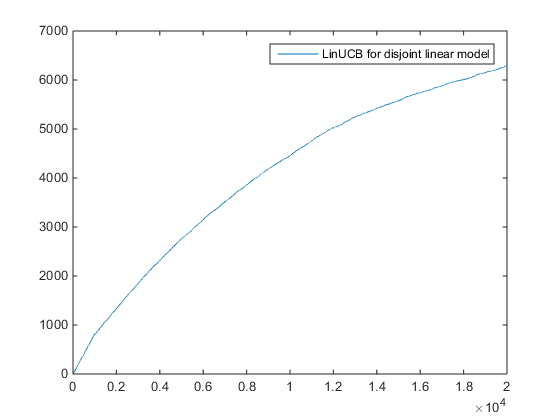
\includegraphics[scale=0.5]{regret-disjoint.png}
	\caption{Regret for disjoint linear model at horizon 20,000 for 1000 arms, with 100 potentially arms pulled at each step, for $\sigma = 1$}
\end{figure}

According to the article, this algorithm approaches a regret of $O(\sqrt{T})$.
%
\\By analyzing the arms pulled, we see that whereas the best arm had an expected reward of 0.7997, the most pulled arm had one of 0.7737, which is quite close, and it was pulled 1094 times. The best potential arm was pulled 683 times.
%
\\The code can be found in \texttt{linUCB\_multipletheta.m}.


\section{Comparison with contextual Thompson Sampling}

\subsection{Thompson Sampling algorithm}

For Thompson Sampling algorithm, an assumption is made on the posterior distribution of $\theta$. Then, at each step $t$ we draw a sample $\widetilde{\theta}_t$ according to this distribution, and pull the arm $a_t$ corresponding to $a_{t} = \mathrm{argmax}_{a_t} \widetilde{\theta}_{t}^{T} x_a$.
%
\\The whole question is now : what model should we take for the posterior probability ? In her thesis, Emilie Kaufmann proposes to take a Gaussian law. Indeed, with a noise $\epsilon_t \sim \mathcal{N}(0,\sigma^2)$, we can draw $\widetilde{\theta}_{t}$ according to the law $\mathcal{N}(\widehat{\theta}_t,v_t^2 A_t^{-1})$ where $\widehat{\theta}_t = A_{t}^{-1}b_{t}$ is the estimate of $\theta$ at step $t$,  $v_t = \sigma \sqrt{9 \: d \: \log \frac{t}{\delta}}$ and $A_t = I_d + D_t^T D_t$, to obtain a confidence interval with probability at least $1-\delta$ in dimension $d$.

\subsection{Results}

With Thompson Sampling, we clearly see the impact of the noise and its variance $\sigma^2$. Indeed, here is the regret achieved for different values of $\sigma^2$ :

\begin{figure}[H]
	\centering
	\noindent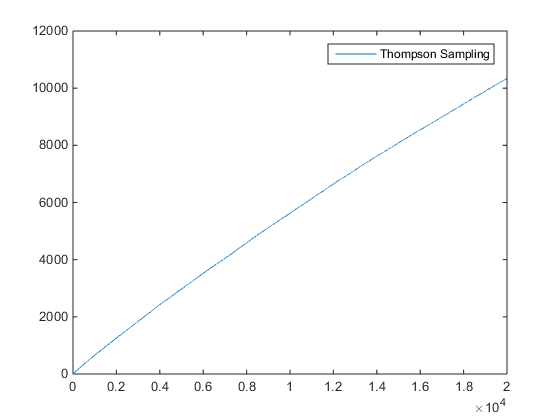
\includegraphics[scale=0.25]{thompson_noise1.png}
	\noindent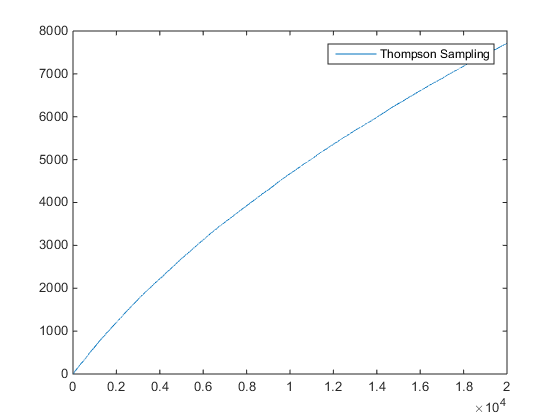
\includegraphics[scale=0.25]{thompson_noise05.png}
	\noindent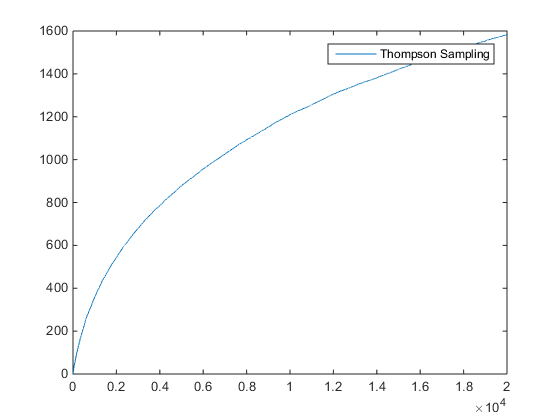
\includegraphics[scale=0.25]{thompson_noise01.png}
	\caption{Left : regret for Thompson Sampling with $\sigma^2 = 1$ - Middle : $\sigma^2 = 0.5$ - Right : $\sigma^2 = 0.1$}
\end{figure}

For  $\sigma^2 = 0.1$, the best arm was effectively the most pulled, and it was pulled 1549 times over 20,000. But for $\sigma^2 = 1$, the most pulled arm was only pulled 83 times, for an expected regret of 0.7433 to be compared with 0.8377 for the best arm. We see that the algorithm is much more imprecise for high value of $\sigma^2$, which seems logical, as we draw $\widehat{\theta}_t$ according to a normal law whose variance directly depends on $\sigma$. 
%
\\The code can be found in \texttt{Thompson.m}.

\section{Analysis of OFUL algorithm}
\subsection{Principle}

OFUL (optimism in the face of uncertainty) is also an optimistic algorithm, because it computes a confidence set for $\theta$, and chooses the arm which maximizes the rewards over all $\hat{\theta}_t$ lying in this confidence set.
%
\\The pseudo code for the OFUL algorithm is:
\\\begin{algorithm}[H]
 \KwData{bandit $\mathcal{A}$, exploration parameter $\alpha$, $K$, horizon $T$}
 $A_1 = I_d$ \;
 $b_1 = 0$ \;
 \For{$t = 1, 2, \ldots, T$}{
  $\hat{\theta}_t = A_t^{-1} b_t$ \;
  Randomly select a set $\mathcal{A}_t \subset \mathcal{A}$ of $K$ arms \;
  
  \For{$a \in \mathcal{A}_t$}{
    $p_{t,a} = \hat{\theta}_t^{\top} x_a + f(t,a)$
   }
   
   Choose arm with higher UCB: $a^*_t = \mathrm{argmax}_{a \in \mathcal{A}_t} p_{t,a} $ \; 
   Observe reward $r_t$ \;
   $A_{t+1} = A_t + x_{a^*_t} x_{a^*_t}^{\top}$ \;
   $b_{t+1} = b_t + r_t x_{a^*_t}$ \;
   }
 
  \KwResult{sequences of actions $(a^*_t)$ and payoffs $(r_t)$, $\hat{\theta}_T$}
 \vspace{5mm}
 \caption{OFUL algorithm}
\end{algorithm}
%
\vspace{5mm}
Computing $f(t,a)$ is the key of the algorithm; it is related to the upper bound on the estimated reward for arm $a$ at time $t$. 
\\We have, according to \textit{Exploring compact
	reinforcement-learning representations with linear regression} $\left[ 3\right]$ , with probability $1 - \delta$,
$$\Vert \hat{\theta}_t - \theta \Vert_{A_t} 
\leq 
\sigma^2 \sqrt{2 \, \mathrm{log} ( \frac{ \vert A_t \vert^{1/2} }{\delta})} + 1$$
Where $\Vert u \Vert_M = \sqrt{u^{\top} M u }$ ($u$ is a $d\times 1$ vector, $M$ is a $d\times d$ symmetric definite positive matrix matrix).
\\If $M$ is invertible, then for all $u, v$ we have $\vert u^{\top} v \vert \leq \Vert u \Vert_M \Vert v \Vert_{M^{-1}}$, because since $M$ is symmetric definite positive, there exists a symmetric definite positive matrix $S$ such that $S^2 = M$, and we have:
 $$\begin{aligned}\vert u^{\top} v \vert &= \vert u^{\top}S^{\top} S^{-1} v \vert 
 \\&\leq \Vert Su \Vert \Vert S^{-1}v \Vert 
 \\&\leq \Vert u \Vert_M \Vert v \Vert_{M^{-1}}
 \end{aligned}$$
If we apply this to $M = A^{-1}_t$ (which is symmetric definite positive because $A_t$ is), $u =x_a$ and $v =  \hat{\theta}_t - \theta$, we get an upper bound on $\vert x_a^{\top} \theta - x_a^{\top} \hat{\theta}_t \vert$ with probability $1-\delta$ : 
$$f(t,a) =  \Vert x_a \Vert_{A^{-1}_t} (\sigma^2 \sqrt{2 \, \mathrm{log} ( \frac{ \vert A_t \vert^{1/2} }{\delta})} + 1)$$
%
\\The code can be found in \texttt{OFUl.m}.

\subsection{Comparison with LinUCB}

Typically, the OFUL algorithm is very similar to linUCB but $\alpha$ is replaced by an adaptive exploration rate. Hence, we obtain a lower regret with OFUL :

\begin{figure}[H]
	\centering
	\noindent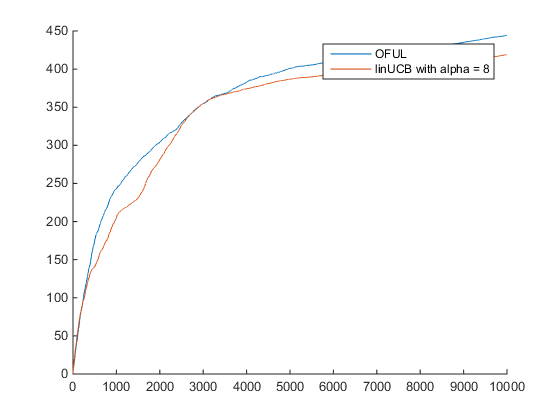
\includegraphics[scale=0.5]{oful.png}
	\caption{Regret for OFUL algorithm}
\end{figure}

The final regret value is here around 400 whereas it was around 200 for linUCB with the best fitted $\alpha$.

The best arm was effectively the most pulled and was pulled 922 times, similar to 944 for linUCB. But, for a given sample, linUCB detects slightly better which arm is the best among the pool.
\\Nevertheless, OFUL was here used with its defaults parameters, and we state in fact that OFUL is very similar to linUCB with $\alpha = 1$.
%
%
\newpage
\begin{thebibliography}{9}

   \bibitem{}
          Lihong Li,
               Wei Chu,
               John Langford,
               Robert E. Schapire,
          \emph{A Contextual-Bandit Approach to Personalized News Article Recommendation}.
          2010.
          
          \bibitem{}
          Wei Chu,
          Lihong Li,
          Lev Reyzin,
          Robert E. Schapire,
          \emph{Contextual Bandits with Linear Payoff Functions}.
          2011.
          
          \bibitem{}
          Thomas J. Walsh, Istvan Szita, Carlos Diuk, Michael L. Littman,
                    \emph{Exploring compact
reinforcement-learning representations with linear regression}.
         2011.
        
        \bibitem{}
        Emilie Kaufmann
        \emph{Analyse de strat�gies bay�siennes et fr�quentistes
        	pour l�allocation s�quentielle de ressources}.
        2014.
        

\end{thebibliography}

\end{document}